\chapter{Abstrake simpliziale Komplexe}
\section{Definiton und geometrische Realisierung}
Um nicht an die geometrische Definition von simplizialen Komplexen
im $\R^d$ gebunden zu sein, abstrahieren wir nun von diesem geometrischen Konzept,
um simpliziale Komplexe rein kombinatorisch und unabhägig von euklidschen Räumen
beschreiben zu können.

\begin{thDef}%
    [Abstrakter simplizialer Komplex, abstraktes Simplex, Dimension, Teilkomplex]%\hfill\\
    Ist $V$ eine Menge und $K\subset\pot{V}$, so dass alle Elemente von $K$
    endliche Mächtigkeit haben, so ist $(V,K)$ ein \emph{abstrakter simplizialer
    Komplex}, falls zusätzlich gilt:
    \[ \forall\,F\in K 
        \;\forall\, F'\subset F \colon\; F'\in K
    \]
    Ein Element $F\in K$ nennen wir \emph{(abstraktes) Simplex} und die
    \emph{Dimension von $F$} ist gegeben durch $\dim(F) \defeq
    \abs{F}-1$.
    Die \emph{Dimension von $K$} ist das Maximum der Dimensionen seiner Simplizes (oder
    $\infty$, falls dieses nicht existiert):
    \[ \dim(K) \defeq \max_{F\in K}\,\dim(F)  \;\in\N\cup\{\infty\} \]
    Ist $\abs{V}$ endlich, so sprechen wir von einem \emph{endlichen
    simplizialen Komplex}. Sind $V'\subset V,$ $K'\subset K$ und definiert
    $(V',K')$ selbst einen simplizialen Komplex, so nennen wir $(V',K')$ einen
    \emph{Teilkomplex von $(V,K)$}.
\end{thDef}

In Zukunft notieren wir anstatt des Paars $(V,K)$ oft nur noch $K$ und
nehmen an, dass $V=\bigcup K$ gilt. Außerdem können wir aus jedem geometrischen
simplizialen Komplex~$\Delta$ einen abstrakten gewinnen, indem wir wie folgt
vorgehen: Sei $V \defeq V(\Delta)$ die Knotenmenge von $\Delta$ und $K$ wie folgt
gegeben:
\[ K \defeq \bigl\{ V_\sigma 
    \Mid V_\sigma \text{ ist Knotenmenge eines Simplex $\sigma\in\Delta$} \bigr\}
\]
Dann ist $(V,K)$ klarerweise ein abstrakter simplizialer Komplex, welchen wir
eine \emph{geometrische Realisierung von $\Delta$} nennen. (Siehe
\cref{asc:fig:geomrealization}.) Das Polyeder $\polyeder\Delta$ bezeichnen wir
dann auch als ein \emph{Polyeder von $K$}.

\begin{figure}
    \centering
    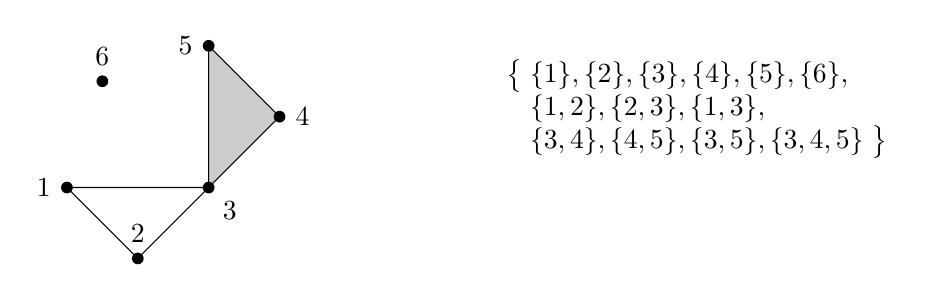
\begin{tikzpicture}[%
        mypoint/.style={shape=circle, inner sep=1.5pt, color=black, fill}
    ]
        \begin{scope}[scale=0.90]
            \coordinate (1) at (0,0);
            \coordinate (2) at (1,-1);
            \coordinate (3) at (2,0);
            \coordinate (4) at (3,1);
            \coordinate (5) at (2,2);
            \coordinate (6) at (0.5,1.5);
            
            \draw (1) -- (2) -- (3) -- cycle;
            \draw [fill=black!20] (3) -- (4) -- (5) -- cycle;
            
            \foreach \n/\ang in 
                {1/left,2/above,3/below right,4/right,5/left,6/above}
                \node [mypoint,label=\ang:$\n$] at (\n) {};
        \end{scope}

        \node [align=left] at (8,1) {%
            $\displaystyle
            \bigl\{\; \{1\}, \{2\}, \{3\}, \{4\}, \{5\}, \{6\},$    \\
            $\displaystyle\hphantom{\bigl\{\;}
                    \{1,2\}, \{2,3\}, \{1,3\},$                     \\
            $\displaystyle\hphantom{\bigl\{\;}
                    \{3,4\}, \{4,5\}, \{3,5\}, \{3,4,5\}
            \;\bigr\}$%
        };
    \end{tikzpicture}
    \caption{Geometrische Realisierung (links) und zugehöriger abstrakter
    simplizialer Komplex (rechts)}
    \label{asc:fig:geomrealization}
\end{figure}

\begin{thBeispiel}[Graphen als abstrakte simpliziale Komplexe]
    Jeder (einfache, ungerichtete) Graph $(\tilde V,E)$ mit
    Knotenmenge~$\tilde V$ und Kantenmenge~$E$ definiert einen
    eindimensionalen simplizialen Komplex~$(V,K)$: Setzte $V\defeq\tilde V$ und
    $K\defeq \{ A \Mid A\subset \{u,v\}\in E \}$. 
    (Siehe \cref{asc:fig:geomrealization}.)
\end{thBeispiel}

\begin{figure}
    \centering
    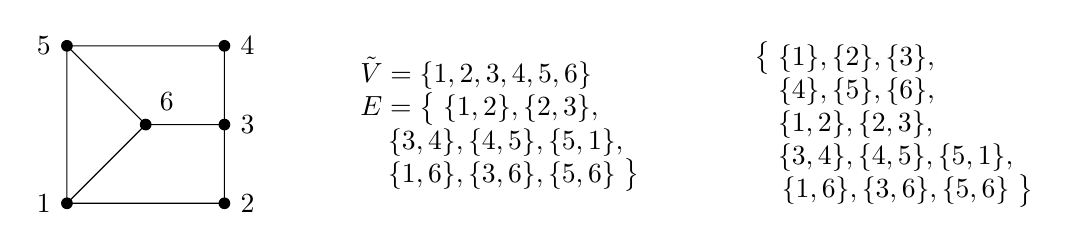
\begin{tikzpicture}[%
            mypoint/.style={shape=circle, inner sep=1.5pt, color=black, fill}
    ]
    \coordinate (1) at (0,0);
    \coordinate (2) at (2,0);
    \coordinate (3) at (2,1);
    \coordinate (4) at (2,2);
    \coordinate (5) at (0,2);
    \coordinate (6) at (1,1);

    \draw (1) \foreach \n in {2,...,6,1,5} { -- (\n) } (6) -- (3);
    \foreach \n/\ang in 
        {1/left,2/right,3/right,4/right,5/left,6/above right}
        \node [mypoint,label=\ang:$\n$] at (\n) {};
        
    \node [align=left] at (5.5,1) {%
        $\displaystyle
            \tilde V = \{ 1,2,3,4,5,6 \}$                       \\
        $\displaystyle
            E = \bigl\{\; 
                \{1,2\}, \{2,3\},$\\
        $\displaystyle\quad
                \{3,4\}, \{4,5\}, \{5,1\},$   \\
        $\displaystyle\quad
                \{1,6\}, \{3,6\}, \{5,6\}
        \;\bigr\}$
    };
    
    \node [align=left] at (10.5,1) {%
        $\displaystyle
        \bigl\{\; \{1\}, \{2\}, \{3\},$         \\
        $\displaystyle\hphantom{\bigl\{\;}
                \{4\}, \{5\}, \{6\},$          \\
        $\displaystyle\hphantom{\bigl\{\;}
                \{1,2\}, \{2,3\},$              \\
        $\displaystyle\hphantom{\bigl\{\;}
                \{3,4\}, \{4,5\}, \{5,1\},$     \\
        $\displaystyle\quad
                \{1,6\}, \{3,6\}, \{5,6\}
        \;\bigr\}$
    };
    \end{tikzpicture}
    \caption{Graph (links), Graph $(\tilde V,E)$ abstrakt (mittig) 
        und zugehöriger abstrakter simplizialer Komplex (rechts)}
    \label{asc:fig:graphtocomplex}
\end{figure}

Man sieht relativ einfach ein, dass jeder endliche simpliziale Komplex $(V,K)$ 
eine geometrische Realisierung im $\R^{\abs{V}-1}$ hat, siehe beispielsweise
Matou\v sek\cite[Ch.\,1,\;1.5]{bookc:matousek03}, oder in einer allgemeineren
Variante Munkres\cite[Ch.\,1,\;\S3,\;3.1]{bookc:munkres84}. Stattdessen
verweisen wir hier auf \cref{asc:geomrealization}, welcher eine schärfere Aussage
liefert.


\section{Dimension geometrischer Realisierungen}
Wir wollen nun folgenden Satz beweisen, welcher uns eine obere Schranke für die
nötige Dimension $d\in\N$ gibt, für welche es zu einem abstrakten simplizalen
Komplex eine geometrische Realisierung im $\R^d$ gibt.

\begin{thSatz}%
    [Satz über die maximal nötige Dimension einer geometrischer Realisierung]
    \label{asc:geomrealization}
    \hfill\\
    %
    Sei $K$ ein endlicher abstrakter simplizaler Komplex der Dimension 
    $\dim(K)=d\in\N$.
    Dann besitzt $K$ eine geometrische Realisierung im $\R^{2d+1}$.
\end{thSatz}

Zum Beweis dieses Satzes benötigen wir noch einige Hilfsmittel. 

\begin{thLemma}[Hinreichende Bedingung für geometrische Realisierung]
    \label{asc:suffprelimgeomrealization}
    %
    Seien $d\in\N,\; (V,K)$ ein abstrakter simplizialer Komplex und
    $f\colon V\to\R^d$ eine injektive Abbildung mit folgender Eigenschaft:
    \[ \forall\,F,G\in K\colon \; f(F\cup G) \text{ ist eine Menge affin
        unabhängiger Vektoren}
    \]
    Dann ist 
    \[ \bigl\{ \conv\bigl(f(F)\bigr) \cMid[\;]\big F\in K \bigr\} \]
    eine geometrische Realisierung von $K$ im $\R^d$.
\end{thLemma}

\begin{proof}
    Es ist nur zu zeigen, dass die zweite Bedingung aus \cref{gsc:def:gsc}
    erfüllt ist (-- der Rest ist klar). Seien dazu $F,G\in K$. 
    Da $f(F\cup G)$ nach Voraussetzung affin unabhängig ist, definiert 
    $\sigma \defeq \conv\bigl(f(F\cup G)\bigr)$ ein Simplex im $\R^d$. 
    Außerdem gilt offenbar $f(F), f(G)\subset f(F\cup G)$, weshalb
    $\conv\bigl(f(F)\bigr)$ und 
    $\conv\bigl(f(G)\bigr)$ Seiten von $\sigma$
    sind. Da die Seiten eines Simplex nach \cref{gsc:complexofsimplex} einen
    simplizialen Komplex bilden, ist auch der Schnitt dieser beiden Seiten 
    eine Seite von $\sigma$, etwa $\conv\bigl(f(T)\bigr)$ für 
    $T\subset F\cup G$. Dann gilt also:
    \[ \conv\bigl(f(F)\bigr) \cap \conv\bigl(f(G)\bigr) 
        = \conv\bigl(f(T)\bigr)
    \]
    Da $f(F\cup G)$ affin unabhängig ist, sieht man schnell ein, dass das Bilden
    der konvexen Hülle über Teilmengen davon eine injektive Operation ist.
    Zusammen mit der gegebenen Injektivität von~$f$ ergibt sich
    $T = F \cap G$, und da letztere Menge sicherlich auch in~$K$ enthalten ist, 
    sind wir fertig.
    \\
\end{proof}

Um nun Abbildungen zu finden, auf die wir \cref{asc:suffprelimgeomrealization}
anwenden können, bedienen wir uns der sogenannten \emph{Momentenkurve} und ihrer
nützlichen Eigenschaften:

\begin{thDef}[Momentenkurve]
    Zu $d\in\N$ ist die \emph{Momentenkurve im $\R^d$} gegeben durch:
    \[  \R \to \R^d, \quad x\mapsto (x,x^2,\ldots,x^d) \]
\end{thDef}

\begin{thLemma}[Eigenschaften der Momentenkurve]
    \label{asc:momentumcurveprop}
    %
    Sei $d\in\N$ und $\gamma$ die Momentenkurve in $\R^d$. Dann hat $\gamma$
    folgende Eigenschaften:
    \begin{enumerate}[a)]
        \item
            Jede (affine) Hyperebene im $\R^d$ schneidet $\gamma$ 
            in maximal~$d$ Punkten.
        \item\label{asc:momentumcurveprop:pointsaffinlyindependent}
            Je $d+1$ Punkte aus $\Image(\gamma)$ sind affin unabhängig.
        \item
            Schneidet eine (affine) Hyperebene $\gamma$ in $d$ verschiedenen 
            Punkten, so wechselt $\gamma$ an jeder dieser Stellen von einem
            durch die Hyperebene gegebenen Halbraum zum anderen.
    \end{enumerate}
\end{thLemma}

\begin{proofsketch}
    Indem man eine die Hyperebene definierende Gleichung und die besondere Form
    der Momentenkurve betrachtet, sieht man, dass sich die Aussagen über
    Schnittpunkte auf algebraische Argumente über Nullstellen von Polynomen
    zurückführen lassen. (Genaueres findet man bei 
    Matou\v sek\cite[Ch.\,1,\;1.6.4]{bookc:matousek03}.)
    \\
\end{proofsketch}

Wir haben nun alles beisammen, um die Hauptaussage dieses Abschnitts beweisen zu
können:
\begin{proof}[Beweis von \cref{asc:geomrealization}]
    Sei also $K$ ein endlicher simplizialer Komplex mit $\dim(K)=d\in\N$.
    Seien außerdem $m\in\N$ und $x_0,\ldots,x_m$ die (verschiedenen) Punkte
    aus $\bigcup K$. Bezeichne weiter $\gamma$ die Momentenkurve im $\R^{2d+1}$.
    Definiere dann eine Abbildung
    $f\colon \bigcup K\to\R^{2d+1}$ für $i\in\setZeroto m$ durch 
    \[ f(x_i) \defeq \gamma(i) 
    . \]
    Es ist $f$ offenbar injektiv und außerdem gilt für alle $F,G\in K$:
    \[ \abs{F\cup G} \leq \abs{F}+\abs{G} \leq (d+1)+(d+1) = 2d+2 \]
    Also sind nach \mycref{asc:momentumcurveprop:pointsaffinlyindependent}
    die Vektoren in $f(F\cup G)$ affin unabhängig und wir können
    \cref{asc:suffprelimgeomrealization} anwenden.
    \\
\end{proof}


\section{Zusammenhang zu partiell geordneten Mengen}
Zur Erinnerung geben wir kurz die folgende Definition:

\begin{thDef}[Partiell geordnete Menge]
    Eine \emph{partiell geordnete Menge $(P,\leq)$} besteht aus einer Menge~$P$
    und einer Relation~$\leq$ auf $P$ mit den folgenden Eigenschaften:
    \begin{enumerate}[a)]
        \item
            Reflexivität:\quad $\forall\, x\in P\colon\; x \leq x$
        \item
            Transitivität:\quad $\forall\, x,y,z\in P\colon 
            (x\leq y \,\wedge\, y\leq z) \implies x \leq z$
        \item
            Anti-Symmetrie:\quad $\forall\, x,y\in P\colon
            (x\leq y \,\wedge\, y\leq x) \implies x = y$
    \end{enumerate}
\end{thDef}

Wir können aus jeder endlichen partiell geordneten Menge einen endlichen 
simplizialen Komplex bilden und umgekehrt.
Folgende Definitionen legen fest, wie wir dies tun wollen:

\begin{thDef}[Ordnungskomplex]
    Ist $(P,\leq)$ eine endliche partiell geordnete Menge, so definieren wir den
    \emph{Ordnungskomplex $\Delta(P)$} wie folgt:
    \[ \Delta(P) \defeq \bigl\{ \{x_1,\ldots,x_k\} \subset P \cMid[\;]\big 
        k\in\N,\; x_1\leq \dots \leq x_k \bigr\}
    \]
    Die Simplizes von $\Delta(P)$ sind also alle endlichen Ketten aus $P$.
\end{thDef}

\begin{thDef}[Partielle Ordnung auf simplizialem Komplex]
    Ist $K$ ein endlicher simplizialer Komplex, so wird
    $K\setminus\{\emptyset\}$ durch die Inklusionsrealtion~$\subset$ partiell
    geordnet. Wir bezeichnen diese zu $K$ assozierte (endliche) 
    partiell geordnete Menge mit $P(K)$.
\end{thDef}

% TODO: kurze Beispiele für beide Operationen
